% 图 2.14 洪特规则给出的 3d 与 4f 离子的 S、L、J 随电子数 n 的变化
\documentclass[tikz,border=5pt]{standalone}
\usetikzlibrary{arrows.meta}
\usepackage{amsmath}
\usepackage{bm}
\usepackage{fontspec}
\setmainfont{Times New Roman}
\usepackage{pgfplots}
\pgfplotsset{compat=1.18}
\begin{document}
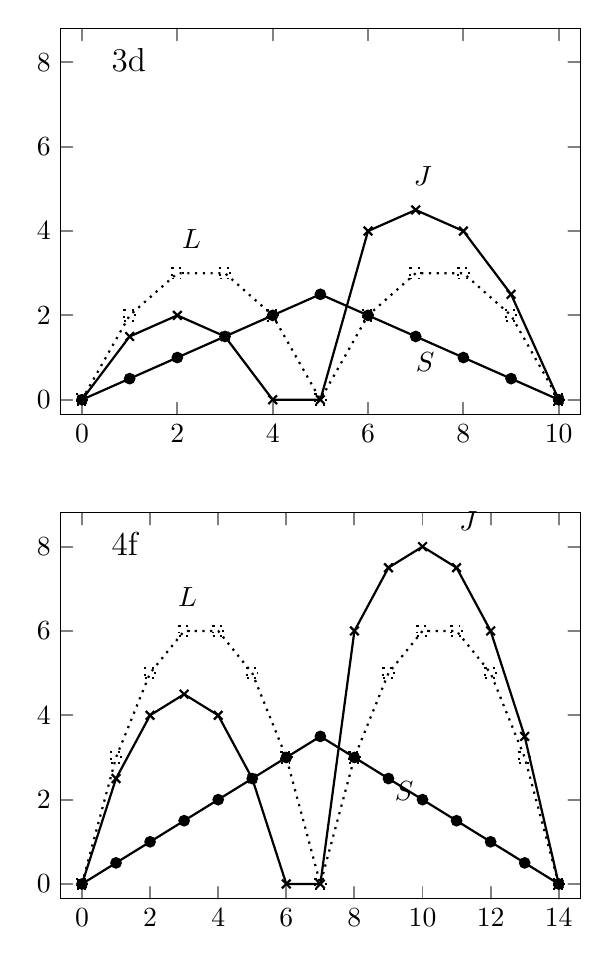
\begin{tikzpicture}[line width=0.8pt,>=Stealth]
% ---------- 3d ----------
\begin{axis}[name=p3,at={(0cm,0cm)},anchor=north west,
  width=6.6cm,height=4.9cm,scale only axis,
  axis lines=box,
  xmin=-0.45,xmax=10.45,ymin=-0.35,ymax=8.8,
  xtick={0,2,4,6,8,10},ytick={0,2,4,6,8},
  tick style={line width=0.7pt,line cap=round},
  clip=false]
  \addplot[sharp plot,dotted,line width=0.8pt,mark=square,mark size=1.9pt,
    mark options={fill=white,line width=0.7pt}]
    coordinates {(0,0)(1,2)(2,3)(3,3)(4,2)(5,0)(6,2)(7,3)(8,3)(9,2)(10,0)};
  \addplot[sharp plot,line width=0.8pt,mark=*,mark size=1.7pt,
    mark options={fill=black}]
    coordinates {(0,0)(1,0.5)(2,1)(3,1.5)(4,2)(5,2.5)(6,2)(7,1.5)(8,1)(9,0.5)(10,0)};
  \addplot[sharp plot,line width=0.8pt,mark=x,mark size=2.2pt,
    mark options={line width=0.8pt}]
    coordinates {(0,0)(1,1.5)(2,2)(3,1.5)(4,0)(5,0)(6,4)(7,4.5)(8,4)(9,2.5)(10,0)};
  \node[anchor=south west,inner sep=1pt] at (axis cs:0.55,7.7) {\large 3d};
  \node[anchor=south] at (axis cs:2.3,3.35) {$L$};
  \node[anchor=south] at (axis cs:7.15,4.85) {$J$};
  \node[anchor=north west] at (axis cs:6.8,1.35) {$S$};
\end{axis}
% ---------- 4f ----------
\begin{axis}[name=p4,at={(0cm,-6.15cm)},anchor=north west,
  width=6.6cm,height=4.9cm,scale only axis,
  axis lines=box,
  xmin=-0.63,xmax=14.63,ymin=-0.35,ymax=8.8,
  xtick={0,2,4,6,8,10,12,14},ytick={0,2,4,6,8},
  tick style={line width=0.7pt,line cap=round},
  clip=false]
  \addplot[sharp plot,dotted,line width=0.8pt,mark=square,mark size=1.9pt,
    mark options={fill=white,line width=0.7pt}]
    coordinates {(0,0)(1,3)(2,5)(3,6)(4,6)(5,5)(6,3)(7,0)(8,3)(9,5)(10,6)(11,6)(12,5)(13,3)(14,0)};
  \addplot[sharp plot,line width=0.8pt,mark=*,mark size=1.7pt,
    mark options={fill=black}]
    coordinates {(0,0)(1,0.5)(2,1)(3,1.5)(4,2)(5,2.5)(6,3)(7,3.5)(8,3)(9,2.5)(10,2)(11,1.5)(12,1)(13,0.5)(14,0)};
  \addplot[sharp plot,line width=0.8pt,mark=x,mark size=2.2pt,
    mark options={line width=0.8pt}]
    coordinates {(0,0)(1,2.5)(2,4)(3,4.5)(4,4)(5,2.5)(6,0)(7,0)(8,6)(9,7.5)(10,8)(11,7.5)(12,6)(13,3.5)(14,0)};
  \node[anchor=south west,inner sep=1pt] at (axis cs:0.77,7.7) {\large 4f};
  \node[anchor=south] at (axis cs:3.1,6.35) {$L$};
  \node[anchor=south] at (axis cs:11.35,8.15) {$J$};
  \node[anchor=north west] at (axis cs:8.9,2.65) {$S$};
\end{axis}
\end{tikzpicture}
\end{document}
